\chapter*{Appendix} 
\label{appendix}
\ifpdf
    \graphicspath{{13_appendix/figures/PNG/}{13_appendix/figures/PDF/}{13_appendix/figures/}}
\else
    \graphicspath{{13_appendix/figures/EPS/}{13_appendix/figures/}}
\fi

\section*{PointNet Model Layers}
\label{appendix-layers}
The model layers and corresponding parameters used in the thesis pipeline (Section \ref{sec:pipeline}, \ref{sec:evaluation}, and \ref{sec:results}) were generated using PyTorch. The following layers were also used for 3D points-based PointNet (Section \ref{sec:additional-3d}
\begin{verbatim}
PointNet(
  (transform): Transform(
    (input_transform): Tnet(
      (conv1): Conv1d(3, 64, kernel_size=(1,), stride=(1,))
      (conv2): Conv1d(64, 128, kernel_size=(1,), stride=(1,))
      (conv3): Conv1d(128, 1024, kernel_size=(1,), stride=(1,))
      (fc1): Linear(in_features=1024, out_features=512, bias=True)
      (fc2): Linear(in_features=512, out_features=256, bias=True)
      (fc3): Linear(in_features=256, out_features=9, bias=True)
      (bn1): BatchNorm1d(64, eps=1e-05, momentum=0.1, affine=True,
                                            track_running_stats=True)
      (bn2): BatchNorm1d(128, eps=1e-05, momentum=0.1, affine=True,
                                            track_running_stats=True)
      (bn3): BatchNorm1d(1024, eps=1e-05, momentum=0.1, affine=True,
                                            track_running_stats=True)
      (bn4): BatchNorm1d(512, eps=1e-05, momentum=0.1, affine=True,
                                            track_running_stats=True)
      (bn5): BatchNorm1d(256, eps=1e-05, momentum=0.1, affine=True,
                                            track_running_stats=True)
    )
    (feature_transform): Tnet(
      (conv1): Conv1d(64, 64, kernel_size=(1,), stride=(1,))
      (conv2): Conv1d(64, 128, kernel_size=(1,), stride=(1,))
      (conv3): Conv1d(128, 1024, kernel_size=(1,), stride=(1,))
      (fc1): Linear(in_features=1024, out_features=512, bias=True)
      (fc2): Linear(in_features=512, out_features=256, bias=True)
      (fc3): Linear(in_features=256, out_features=4096, bias=True)
      (bn1): BatchNorm1d(64, eps=1e-05, momentum=0.1, affine=True,
                                         track_running_stats=True)
      (bn2): BatchNorm1d(128, eps=1e-05, momentum=0.1, affine=True,
                                         track_running_stats=True)
      (bn3): BatchNorm1d(1024, eps=1e-05, momentum=0.1, affine=True,
                                         track_running_stats=True)
      (bn4): BatchNorm1d(512, eps=1e-05, momentum=0.1, affine=True,
                                         track_running_stats=True)
      (bn5): BatchNorm1d(256, eps=1e-05, momentum=0.1, affine=True,
                                         track_running_stats=True)
    )
    (conv1): Conv1d(3, 64, kernel_size=(1,), stride=(1,))
    (conv2): Conv1d(64, 128, kernel_size=(1,), stride=(1,))
    (conv3): Conv1d(128, 1024, kernel_size=(1,), stride=(1,))
    (bn1): BatchNorm1d(64, eps=1e-05, momentum=0.1, affine=True,
                                         track_running_stats=True)
    (bn2): BatchNorm1d(128, eps=1e-05, momentum=0.1, affine=True,
                                         track_running_stats=True)
    (bn3): BatchNorm1d(1024, eps=1e-05, momentum=0.1, affine=True,
                                         track_running_stats=True)
  )
  (fc1): Linear(in_features=1024, out_features=512, bias=True)
  (fc2): Linear(in_features=512, out_features=256, bias=True)
  (fc3): Linear(in_features=256, out_features=2, bias=True)
  (bn1): BatchNorm1d(512, eps=1e-05, momentum=0.1, affine=True,
                                    track_running_stats=True)
  (bn2): BatchNorm1d(256, eps=1e-05, momentum=0.1, affine=True,
                                    track_running_stats=True)
  (dropout): Dropout(p=0.3, inplace=False)
  (logsigmoid): LogSigmoid()
)
\end{verbatim}

The following model summary describes the model used for the 4D PointNet experiment (Section \ref{sec:additional-4d}). 
\begin{verbatim}
PointNet(
  (transform): Transform(
    (input_transform): Tnet(
      (conv1): Conv1d(4, 64, kernel_size=(1,), stride=(1,))
      (conv2): Conv1d(64, 128, kernel_size=(1,), stride=(1,))
      (conv3): Conv1d(128, 1024, kernel_size=(1,), stride=(1,))
      (fc1): Linear(in_features=1024, out_features=512, bias=True)
      (fc2): Linear(in_features=512, out_features=256, bias=True)
      (fc3): Linear(in_features=256, out_features=16, bias=True)
      (bn1): BatchNorm1d(64, eps=1e-05, momentum=0.1, affine=True,
                                         track_running_stats=True)
      (bn2): BatchNorm1d(128, eps=1e-05, momentum=0.1, affine=True,
                                         track_running_stats=True)
      (bn3): BatchNorm1d(1024, eps=1e-05, momentum=0.1, affine=True,
                                        track_running_stats=True)
      (bn4): BatchNorm1d(512, eps=1e-05, momentum=0.1, affine=True,
                                        track_running_stats=True)
      (bn5): BatchNorm1d(256, eps=1e-05, momentum=0.1, affine=True,
                                        track_running_stats=True)
    )
    (feature_transform): Tnet(
      (conv1): Conv1d(64, 64, kernel_size=(1,), stride=(1,))
      (conv2): Conv1d(64, 128, kernel_size=(1,), stride=(1,))
      (conv3): Conv1d(128, 1024, kernel_size=(1,), stride=(1,))
      (fc1): Linear(in_features=1024, out_features=512, bias=True)
      (fc2): Linear(in_features=512, out_features=256, bias=True)
      (fc3): Linear(in_features=256, out_features=4096, bias=True)
      (bn1): BatchNorm1d(64, eps=1e-05, momentum=0.1, affine=True,                                              track_running_stats=True)
      (bn2): BatchNorm1d(128, eps=1e-05, momentum=0.1, affine=True,                                             track_running_stats=True)
      (bn3): BatchNorm1d(1024, eps=1e-05, momentum=0.1, affine=True,                                            track_running_stats=True)
      (bn4): BatchNorm1d(512, eps=1e-05, momentum=0.1, affine=True,                                             track_running_stats=True)
      (bn5): BatchNorm1d(256, eps=1e-05, momentum=0.1, affine=True,                                             track_running_stats=True)
    )
    (conv1): Conv1d(4, 64, kernel_size=(1,), stride=(1,))
    (conv2): Conv1d(64, 128, kernel_size=(1,), stride=(1,))
    (conv3): Conv1d(128, 1024, kernel_size=(1,), stride=(1,))
    (bn1): BatchNorm1d(64, eps=1e-05, momentum=0.1, affine=True,                                              track_running_stats=True)
    (bn2): BatchNorm1d(128, eps=1e-05, momentum=0.1, affine=True,                                             track_running_stats=True)
    (bn3): BatchNorm1d(1024, eps=1e-05, momentum=0.1, affine=True,                                            track_running_stats=True)
  )
  (fc1): Linear(in_features=1024, out_features=512, bias=True)
  (fc2): Linear(in_features=512, out_features=256, bias=True)
  (fc3): Linear(in_features=256, out_features=2, bias=True)
  (bn1): BatchNorm1d(512, eps=1e-05, momentum=0.1, affine=True,                                                 track_running_stats=True)
  (bn2): BatchNorm1d(256, eps=1e-05, momentum=0.1, affine=True,                                                 track_running_stats=True)
  (dropout): Dropout(p=0.3, inplace=False)
  (logsigmoid): LogSigmoid()
)
\end{verbatim}

\section*{Model with No Feature Engineering}
\label{appendix-no-fe}

The model was trained without any feature engineering, and results were collected from hard voting. Table \ref{tab:no_fe_classification_report} indicates that the model was able to perfectly identify and classify event timeslices. However, it was not able to identify and label a single noise timeslice. So, despite the perfect recall for \texttt{class\_1}, the model shows no learning ability. This is further confirmed by the Precision-Recall (PR) and Receiver Operating Characteristic (ROC) Curve in Figure \ref{fig:ncm_no_fe}. The ROC plot shows curves through the diagonal, indicating that the classifier was completely random and learnt nothing. The PR curve for \texttt{class\_1} is also through the diagonal, indicating that its performance was equivalent to a model with no skill. The model could in a different instance predict the reverse, ie., perfectly classify noise and none of the event timeslices.

\begin{table} [ht!]
    \centering
    \begin{tabular}{l c c c c}
    \hline
    \multicolumn{5}{c}{Hard Voting Results: \texttt{(x y time), (x z time) (y z time)}} \\
    \hline
                     & precision & recall & F1-score & support \\
        \texttt{class\_0} & 0.00 &  0.00    & 0.00 & 40\\
        \texttt{class\_1} & 0.50 &  1.00    & 0.67 & 40\\
    \hline
    \end{tabular}
    \caption{No Feature Engineering: Classification Report for \texttt{class\_0} and \texttt{class\_1}}
    \label{tab:no_fe_classification_report}
\end{table}


\begin{figure}
    \centering
    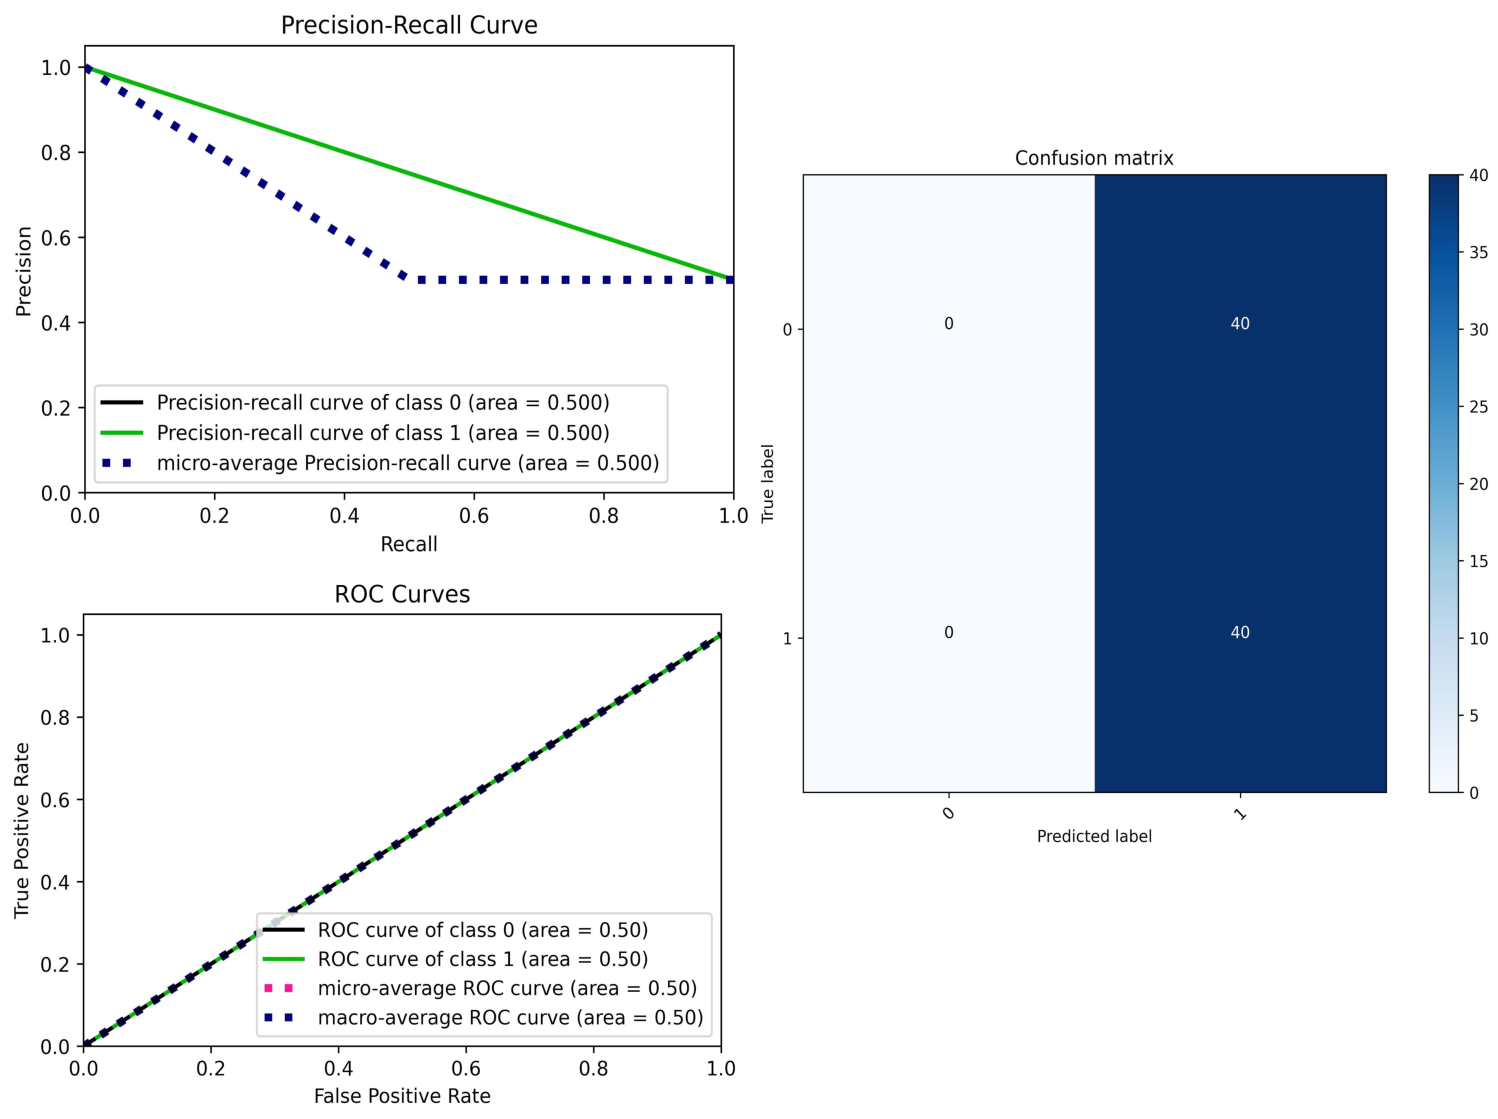
\includegraphics[width=\textwidth, keepaspectratio]{no_fe_metrics.pdf}
    \caption{Classification Metrics: Model without Feature Engineering}
    \label{fig:ncm_no_fe}
\end{figure}




\let\cleardoublepage\clearpage